\documentclass[leqno]{article}
\usepackage[a4paper, margin=1.3in]{geometry}
\usepackage[utf8]{inputenc}
\usepackage{amsmath}
\usepackage{graphicx}
\usepackage{caption}
\usepackage{subcaption}
\usepackage{float}

\title{MAC0210 - Exercício-Programa 2}
\author{Vinicius Agostini - 4367487}
\date{June 2020}

\begin{document}

\maketitle

\section{O Programa}
Segue descrição de cada \textbf{function file} implementado para a
resolução deste exercício-programa.

\subsection{compress(originalImg, k)}
Responsável por realizar a compressão de uma imagem por um fator de compressão
$k$ como especificado no enunciado, isto é, removendo todas as linhas e colunas
com índice $i$ tal que $i \not\equiv 0 \mod k+1$. Assim, supondo que a imagem
original tenha tamanho $p \times p$, o tamanho da imagem comprimida será
$n \times n$, de forma que $p = n + (n-1)k$.

A implementação em Octave se dá selecionando as colunas e linhas usando ranges
com step igual a $k+1$.

\subsubsection{Parâmetros}
\begin{itemize}
    \item \textbf{originalImg} - path para a imagem original a ser comprimida
    \item \textbf{k} - fator de compressão
\end{itemize}

\subsubsection{Saída}
A função gera uma imagem que será salva com o nome \textbf{compressed.png}.

\subsection{decompress(compressedImg, method, k, h)}
Esta função é responsável pela descompressão da imagem com fator de descompressão
$k$ e tamanho dos quadrados interpolantes $h$.

A depender do parâmetro \textbf{method}, a interpolação dos pontos
adicionados no passo anterior é feita a partir dos métodos \textbf{bilinear} ou
\textbf{bicúbico}, também definidos mais adiante em suas próprias funções para
facilitar o entendimento do código.

Em ambos os métodos de interpolação o primeiro passo é expandir a
imagem comprimida inserindo $k$ linhas entre cada par de linhas e $k$ colunas
entre cada par de colunas, fazendo com que a imagem tenha tamanho $p \times p$
novamente. Esse passo é realizado através da função \textbf{expand}, definida
adiante.


\subsubsection{Parâmetros}
\begin{itemize}
    \item \textbf{compressedImg} - path para a imagem comprimida a ser utilizada
    \item \textbf{method} - método de interpolação a ser usado
    \begin{itemize}
        \item \textbf{1} - Bilinear
        \item \textbf{2} - Bicúbico
    \end{itemize}
    \item \textbf{k} - taxa de descompressão
    \item \textbf{h} - tamanho do lado dos quadrados interpolantes como definido
                        no enunciado
\end{itemize}

\subsubsection{Saída}
Gera uma imagem que é salva com o nome de \textbf{decompressed.png}.


\subsection{calculateError(originalImg, decompressedImg)}
Responsável por calcular o erro entre a imagem original e a imagem descomprimida
como definido no enunciado. Aqui é tomado um cuidado extra para calcular o erro
de imagens preto e branco que tem forma $p \times p \times 1$ ao invés de 
$p \times p \times 3$ como imagens coloridas.




\subsection{expand(compressedImg, k)}
Essa função auxiliar é responsável por expandir uma imagem comprimida para o
tamanho original inserindo $k$ linhas e colunas entre cada uma das $n$ linhas
e colunas da imagem comprimida.
A implementação foi criar uma nova imagem de tamanho $p = n + (n-1)k$ e preencher
as posições correspondentes à imagem comprimida, deixando as posições novas com
um valor padrão de zero.

\subsubsection{Parâmetros}
\begin{itemize}
    \item \textbf{compressedImg} - matriz que representa a imagem a ser expandida
    \item \textbf{k} - taxa de descompressão
\end{itemize}

\subsubsection{Saída}
Uma matriz de tamanho $p = n + (n-1)k$ em que apenas as posições correspondentes
à imagem comprimida estão preenchidas.

\subsection{bilinear(compressedImg, k, h)}
Aqui aplicamos a interpolação bilinear por partes, da seguinte maneira: seja
$Q_{ij}$ o quadrado de pontos conhecidos da imagem com canto superior esquerdo
em $(x_i, y_j)$, todos os pontos dentro de $Q_{ij}$ são interpolados pelos
quatro pontos que definem o quadrado, como definido no enunciado.


Vamos discutir a implementação e como otimizar ligeiramente o código se aproveitando
de operações com vetores para utilizar o Octave do jeito que ele funciona melhor.

Seja $p_{ij}(x,y) = a_0 + a_1(x - x_i) + a_2(y - y_j) + a_3(x - x_i)(y - y_j)$,
o nosso polinômio interpolante, podemos notar que, como os pontos da nossa imagem
estão igualmente espaçados, podemos representar as expressões $(x - x_i)$ e
$(y - y_j)$ num vetor de $k+2$ elementos que dividem o intervalo $[0, h]$ igualmente. 

Com um pouco de álgebra linear, podemos chegar na seguinte fórmula matricial para
interpolar todos os valores pertencentes a um mesmo quadrado $Q_{ij}$ de uma só
vez:

$$ p(\forall(x_i, y_j) \in Q_{ij}) = \left( \begin{bmatrix}
       1   & 0      \\
    \vdots & \vdots \\
       1   & h
    \end{bmatrix}
    \begin{bmatrix}
        a_0   & a_1      \\
        a_2   & a_3
     \end{bmatrix} 
     \begin{bmatrix}
        1  & \ldots   & 1    \\
        0  & \ldots   & h
     \end{bmatrix}\right)^T
    $$

Podemos então iterar sobre todos os possíveis quadrados $Q_{ij}$, encontrar a
matriz de coeficientes $a_i$ através da fórmula do enunciado e calcular todos
os pontos em seu interior a partir de operações matriciais.

\subsubsection{Parâmetros}
Os parâmetros de \textbf{decompress} são repassados para \textbf{bilinear},
exceto pelo método de interpolação.

\subsubsection{Saída}
A função devolve uma matriz representando a imagem intepolada, mas deixa a
responsabilidade de salvar esta imagem para a função \textbf{decompress}.


\subsection{bicubic(compressedImg, k, h)}
A aplicação da interpolação bicúbica por partes é bastante semelhante à bilinear,
porém, utilizando mais informação já que para cada um dos quatro cantos que
definem um quadrado $Q_{ij}$, levamos em conta uma aproximação de suas derivadas
a partir do método de diferenças finitas, como definido no enunciado. Nos pontos
de borda o erro naturalmente fica com uma perspectiva pior, por ser necessário
utilizar diferença unilateral ao invés de diferença centralizada.

Novamente a ideia foi tentar aproveitar o poder do Octave realizando o máximo
de operações matriciais quanto fosse possível, e podemos utilizar a mesma
observação do caso bilinear para chegar na seguinte fórmula:

$$ p(\forall(x_i, y_j) \in Q_{ij}) = \begin{bmatrix}
    1   &    0   &    0   &    0     \\
 \vdots & \vdots & \vdots & \vdots   \\ 
    1   &    h   &   h^2  &   h^3
 \end{bmatrix}
 \begin{bmatrix}
     a_{00}   & a_{01} & a_{02} & a_{03}      \\
     a_{10}   & a_{11} & a_{12} & a_{13}      \\
     a_{20}   & a_{21} & a_{22} & a_{23}      \\
     a_{30}   & a_{31} & a_{32} & a_{33}     
  \end{bmatrix} 
  \begin{bmatrix}
     1  & \ldots   & 1      \\
     0  & \ldots   & h      \\
     0  & \ldots   & h^2    \\
     0  & \ldots   & h^3    \\
  \end{bmatrix} $$

Novamente deve-se iterar sobre todos os possíveis quadrados $Q_{ij}$, encontrar a
matriz de coeficientes $a_i$ através da fórmula do enunciado e calcular todos
os pontos em seu interior a partir de operações matriciais.

\subsubsection{Parâmetros}
Os parâmetros de \textbf{decompress} são repassados para \textbf{bicubic},
exceto pelo método de interpolação.

\subsubsection{Saída}
A função devolve uma matriz representando a imagem intepolada, mas deixa a
responsabilidade de salvar esta imagem para a função \textbf{decompress}.


\section{O Zoológico}

\subsubsection*{Imagens preto e branco}

\begin{figure}[H]
    \centering
    \begin{subfigure}{.33\textwidth}
      \centering
      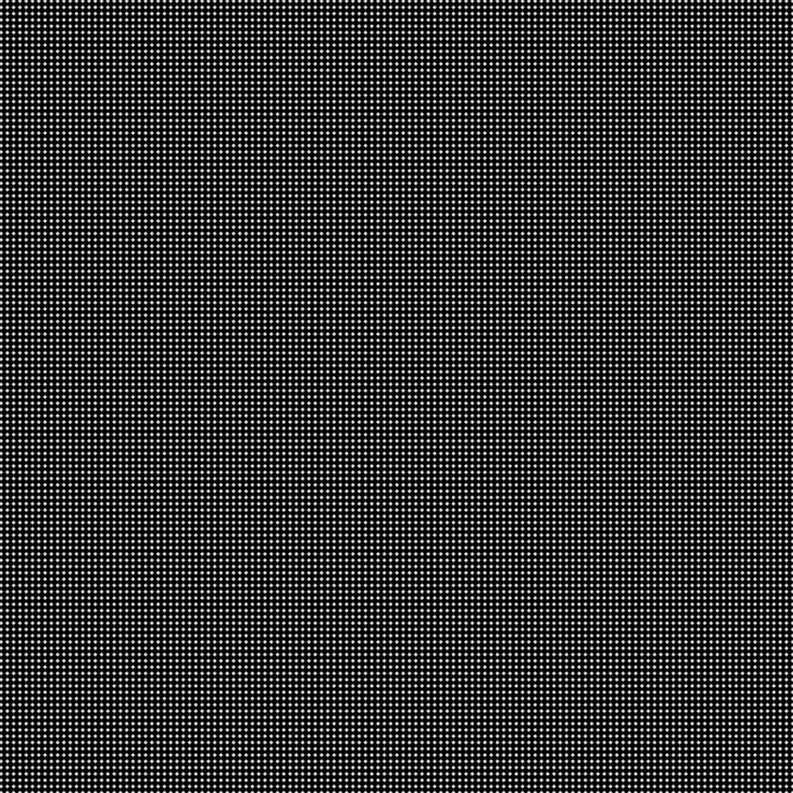
\includegraphics[width=.7\linewidth]{../images/func_1.png}
      \caption{Imagem original  (901x901) }
      \label{fig:sub1}
    \end{subfigure}%
    \begin{subfigure}{.33\textwidth}
      \centering
      
\includegraphics[width=.7\linewidth]{../images/func_1_bil.png}
      \caption{Método bilinear com $k = 3$}
      \label{fig:sub2}
    \end{subfigure}
    \begin{subfigure}{.33\textwidth}
        \centering
        
\includegraphics[width=.7\linewidth]{../images/func_1_bic.png}
        \caption{Método bicúbico com $k = 3$}
        \label{fig:sub1}
      \end{subfigure}%
    \caption{$f(x,y) = (\sin(x) - sin(y))/2$ \\ Erro: 0.68525 e 0.68240}
    \label{fig:test}
\end{figure}

\begin{figure}[H]
    \centering
    \begin{subfigure}{.33\textwidth}
      \centering
      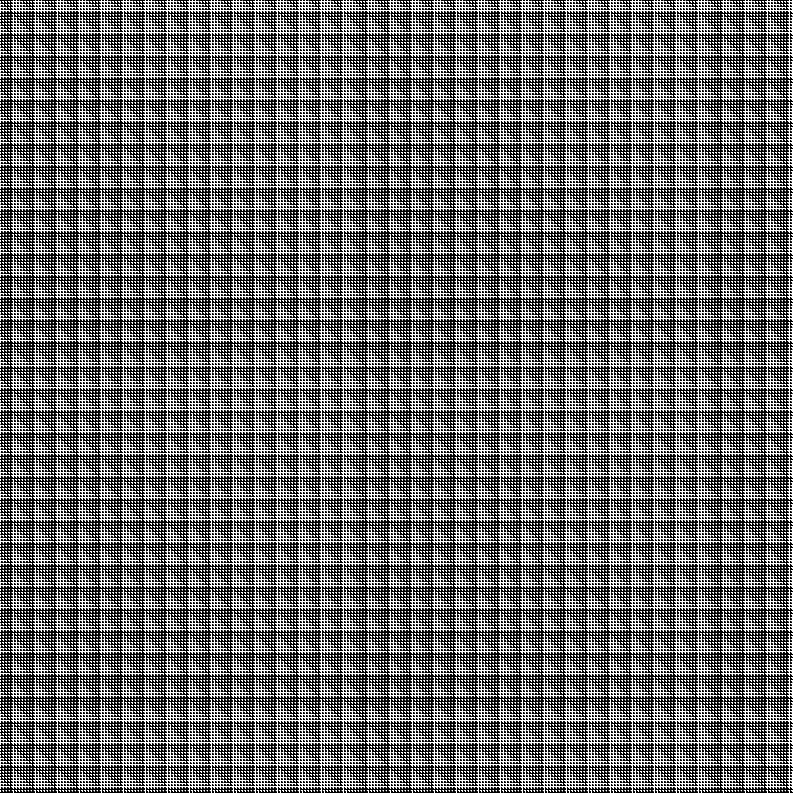
\includegraphics[width=.7\linewidth]{../images/func_2.png}
      \caption{Imagem original  (793x793) }
      \label{fig:sub1}
    \end{subfigure}%
    \begin{subfigure}{.33\textwidth}
      \centering
      
\includegraphics[width=.7\linewidth]{../images/func_2_bil.png}
      \caption{Método bilinear com $k = 3$}
      \label{fig:sub2}
    \end{subfigure}
    \begin{subfigure}{.33\textwidth}
        \centering
        
\includegraphics[width=.7\linewidth]{../images/func_2_bic.png}
        \caption{Método bicúbico com $k = 3$}
        \label{fig:sub1}
      \end{subfigure}%
    \caption{$f(x,y) = \tan(x) - \tan(y)$ \\ Erro: 0.61875 e 0.65526}
    \label{fig:test}
\end{figure}

\subsubsection*{Imagens coloridas}

\begin{figure}[H]
    \centering
    \begin{subfigure}{.33\textwidth}
      \centering
      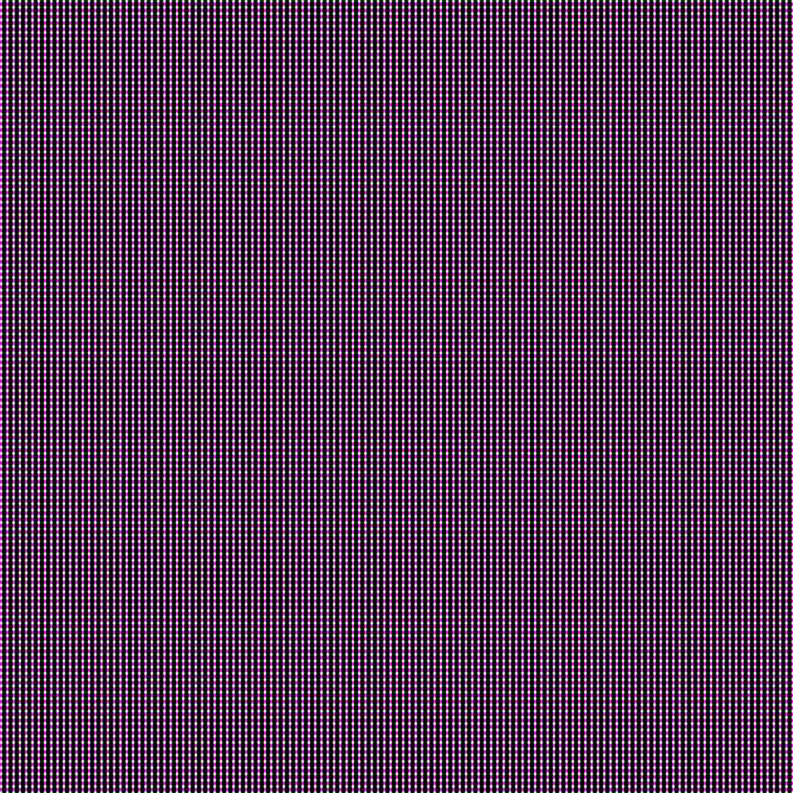
\includegraphics[width=.7\linewidth]{../images/func_1_color.png}
      \caption{Imagem original  (793x793) }
      \label{fig:sub1}
    \end{subfigure}%
    \begin{subfigure}{.33\textwidth}
      \centering
      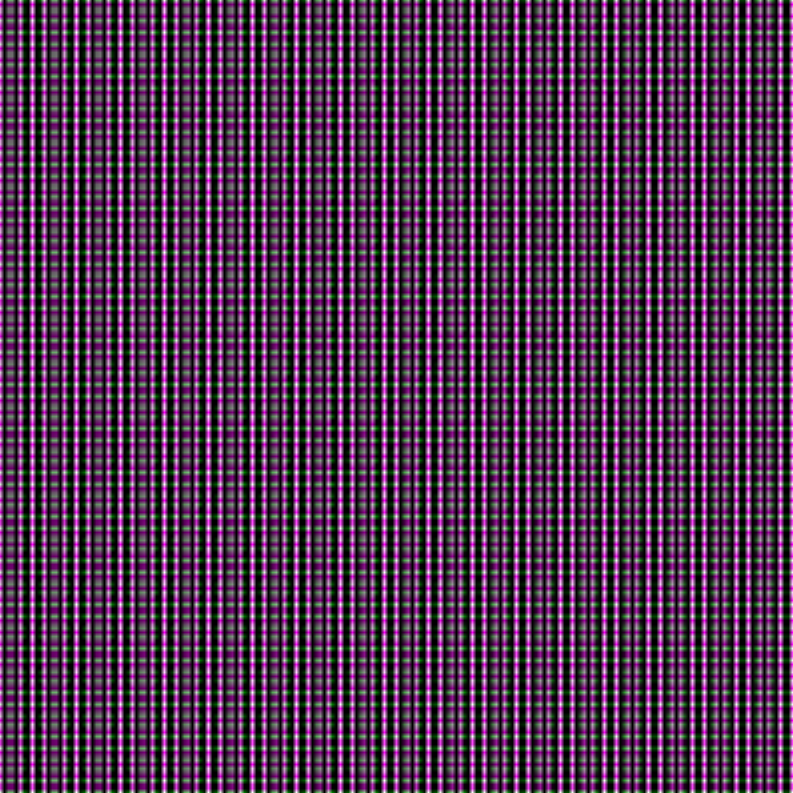
\includegraphics[width=.7\linewidth]{../images/func_1_color_bil.png}
      \caption{Método bilinear com $k = 3$}
      \label{fig:sub2}
    \end{subfigure}
    \begin{subfigure}{.33\textwidth}
        \centering
        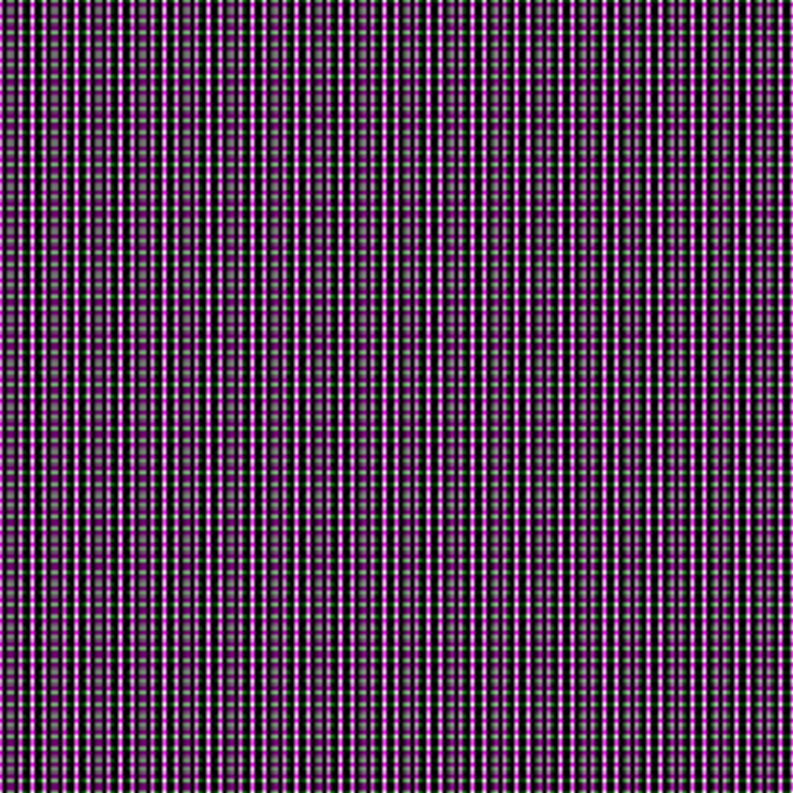
\includegraphics[width=.7\linewidth]{../images/func_1_color_bic.png}
        \caption{Método bicúbico com $k = 3$}
        \label{fig:sub1}
      \end{subfigure}%
    \caption{$f(x,y) = (\sin(x), \frac{\sin(y) + \sin(x)}{2}, \sin(x))$ \\ Erro: 0.76810 e 0.77987}
    \label{fig:test}
\end{figure}

\begin{figure}[H]
    \centering
    \begin{subfigure}{.33\textwidth}
      \centering
      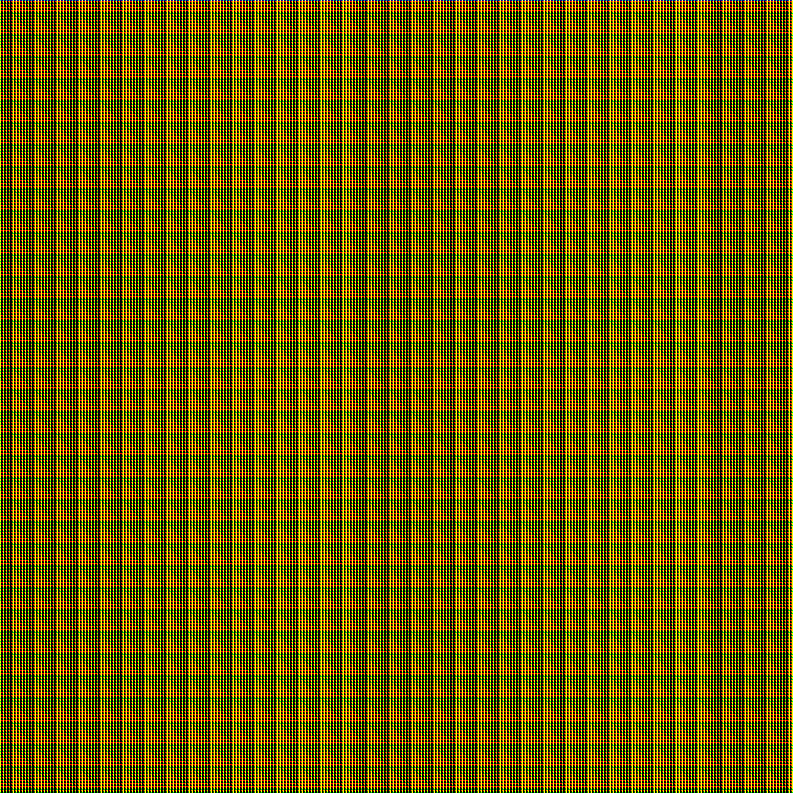
\includegraphics[width=.7\linewidth]{../images/func_2_color.png}
      \caption{Imagem original  (793x793) }
      \label{fig:sub1}
    \end{subfigure}%
    \begin{subfigure}{.33\textwidth}
      \centering
      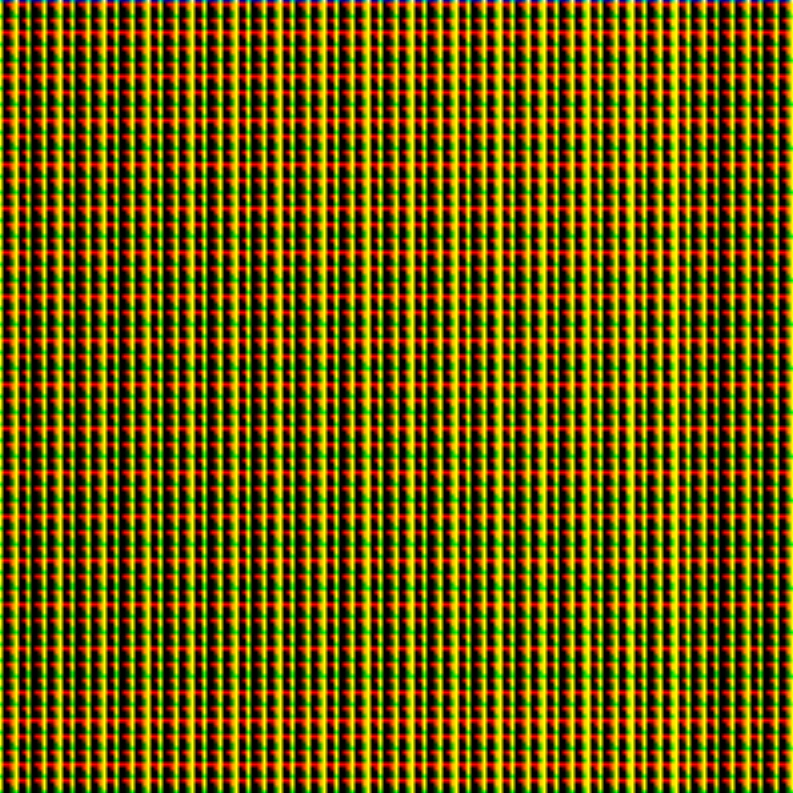
\includegraphics[width=.7\linewidth]{../images/func_2_color_bil.png}
      \caption{Método bilinear com $k = 3$}
      \label{fig:sub2}
    \end{subfigure}
    \begin{subfigure}{.33\textwidth}
        \centering
        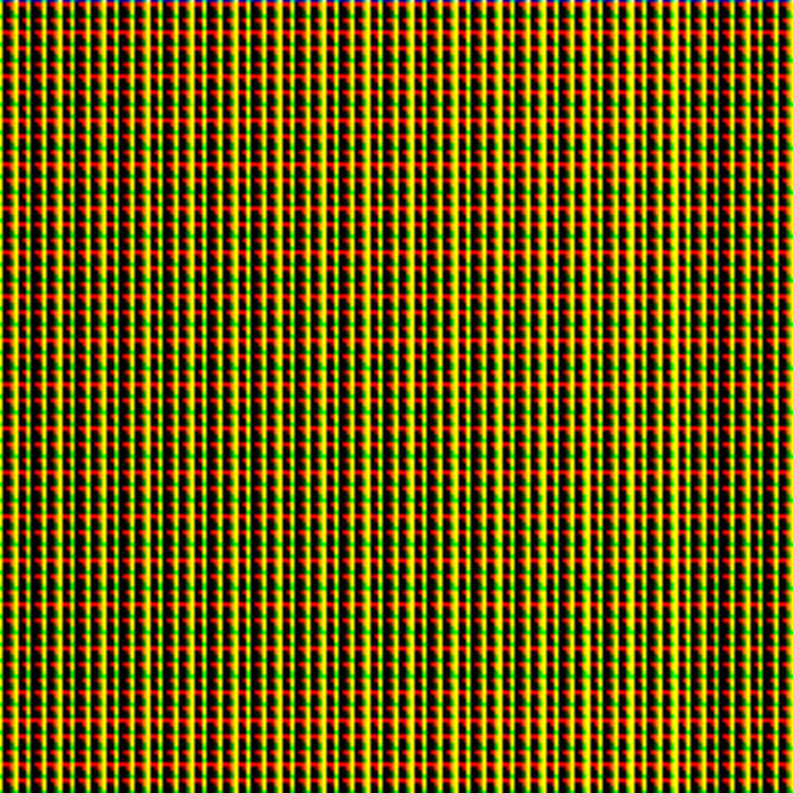
\includegraphics[width=.7\linewidth]{../images/func_2_color_bic.png}
        \caption{Método bicúbico com $k = 3$}
        \label{fig:sub1}
      \end{subfigure}%
    \caption{$f(x,y) = (\tan(x) - \tan(y), \tan(x), \tan(y) - y)$ \\ Erro: 0.82807 e 0.88049}
    \label{fig:test}
\end{figure}

\begin{itemize}
    \item \textbf{Funciona bem para imagens preto e branco?} \\
        Para os testes com imagens geradas a partir de funções, os resultados
        com imagens preto e branco foram um pouco decepcionantes pois esperava
        resultados melhores que para imagens reais, o que não aconteceu.

    \item \textbf{Funciona bem para imagens coloridas?} \\
        Novamente os testes foram um pouco decepcionantes pois para imagens coloridas geradas
        a partir de funções e os resultados foram ainda piores, na casa de 0.8 a 0.9.

    \item \textbf{Funciona bem para todas as funções de classe $C^2$?} \\
        Nos meus testes não consegui gerar imagens a partir de funções com resultados
        que fossem significativamente melhores do que os apresentados e como não
        foi um resultado bom, acredito que não funciona para todas.

    \item \textbf{E para funções que não são de classe $C^2$?} \\
        Os resultados foram bastante semelhantes entre os dois testes para
        imagens preto e branco. Como os resultados não foram bons, acredito
        que não funcione para todas também.

    \item \textbf{Como o valor de h muda a interpolação?} \\
        Testei com diversos valores de $h$ e o erro não mudou significativamente.
    
    \item \textbf{Como se comporta o erro?} \\
        O erro aumentou um pouco em alguns casos conforme $k$ aumentou, se manteve praticamente
        estável conforme $h$ variou, e de forma geral foi um pouco maior para imagens
        coloridas. Acredito que o erro relativamente grande nessas imagens geradas por funções
        pode ser devido a mudanças bruscas na cor, como podemos observar nas imagens,
        não há uma suavidade nas transições como existe em imagens reais.
        
        \begin{figure}[H]
          \centering
          \begin{subfigure}{.45\textwidth}
            \centering
            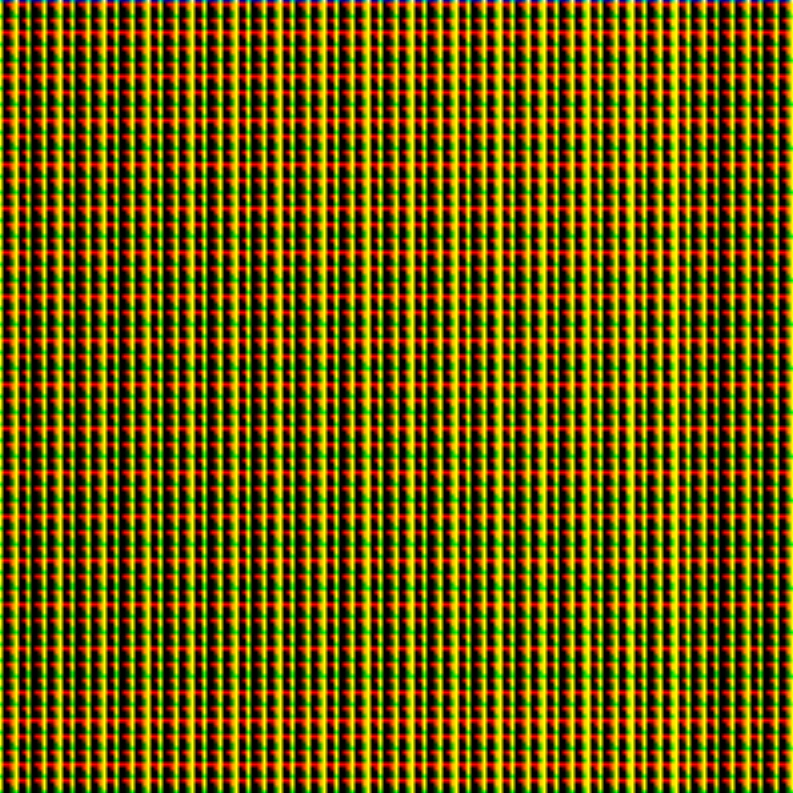
\includegraphics[width=.7\linewidth]{../images/func_2_color_k3.png}
            \caption{Método bilinear com $k = 3$}
            \label{fig:sub2}
          \end{subfigure}
          \begin{subfigure}{.45\textwidth}
              \centering
              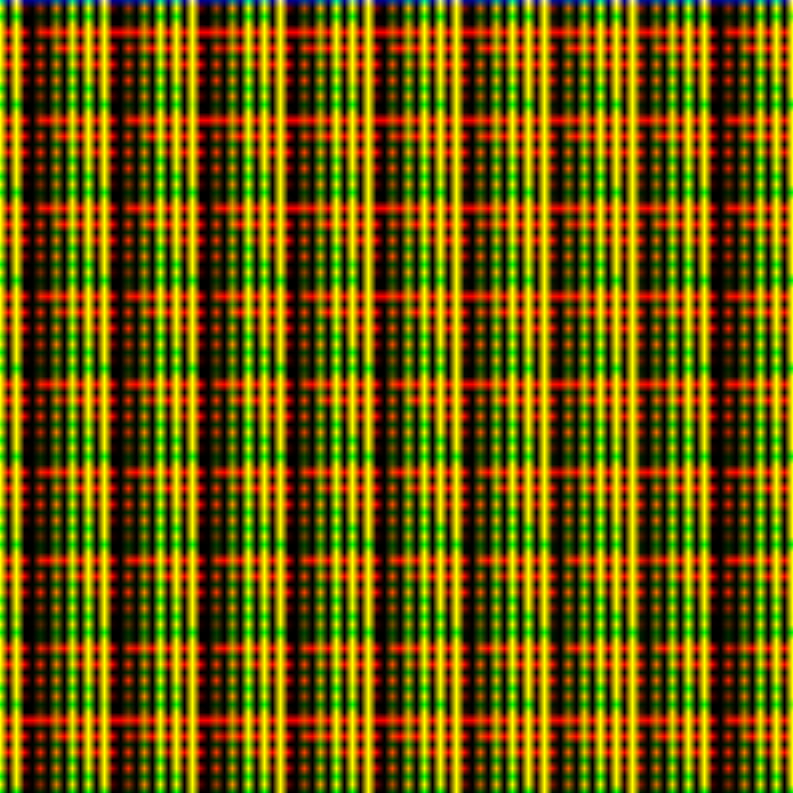
\includegraphics[width=.7\linewidth]{../images/func_2_color_k7.png}
              \caption{Método bilinear com $k = 7$}
              \label{fig:sub1}
            \end{subfigure}%
          \caption{Erro: 0.82807 e 1.0045}
          \label{fig:test}
      \end{figure}

    \item \textbf{Comparação $k = 7$ e $k = 1$ três vezes} \\
        O erro ficou muito parecido em ambos os casos nos meus testes, até mesmo
        iguais em alguns testes. Segue um exemplo:

        \begin{figure}[H]
            \centering
            \begin{subfigure}{.45\textwidth}
              \centering
              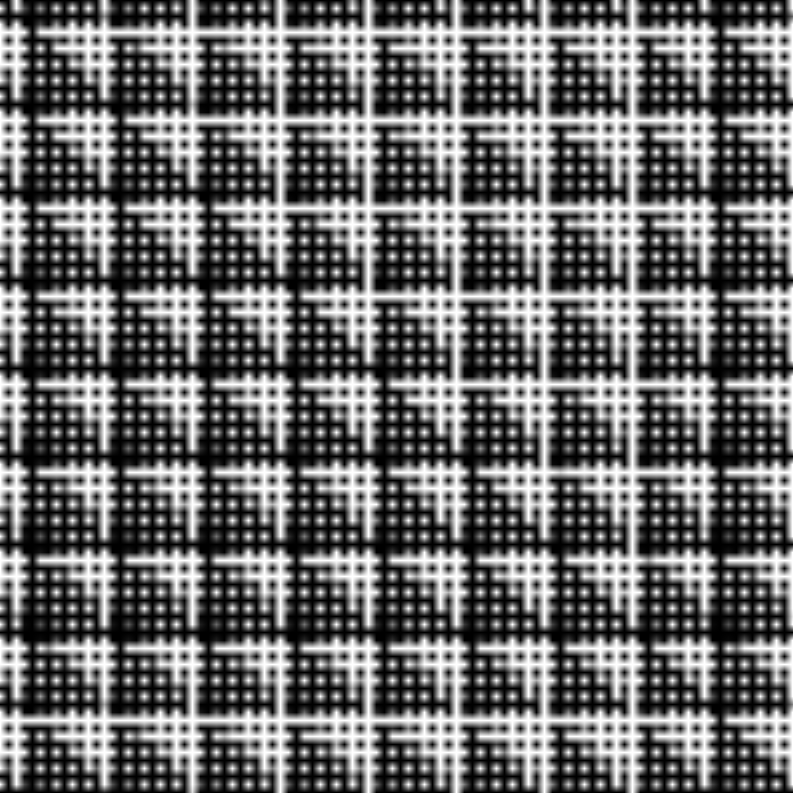
\includegraphics[width=.7\linewidth]{../images/func_2_k7x1_bil.png}
              \caption{Método bilinear com $k = 7$}
              \label{fig:sub2}
            \end{subfigure}
            \begin{subfigure}{.45\textwidth}
                \centering
                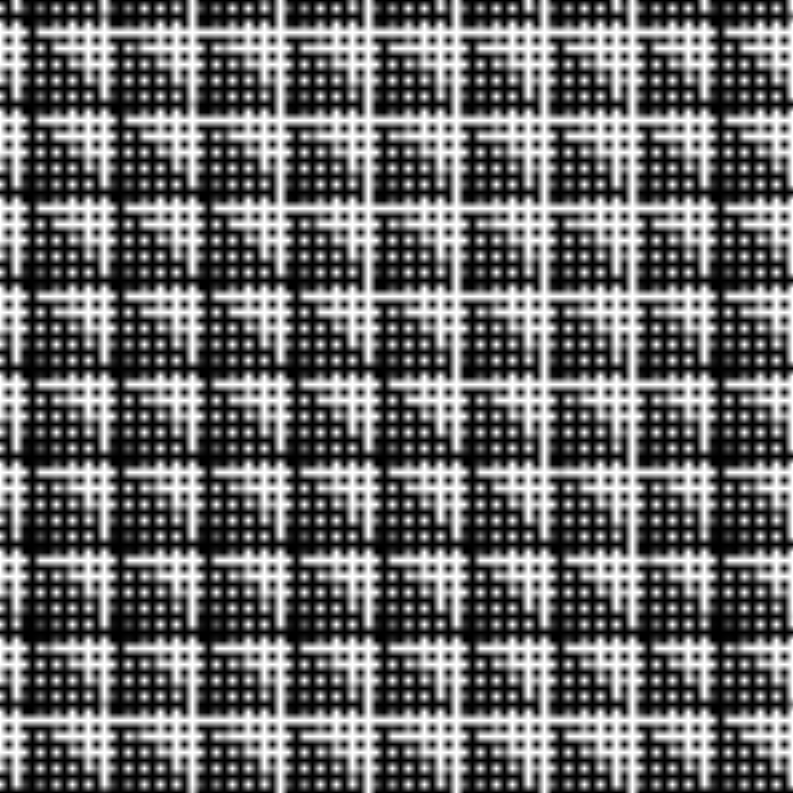
\includegraphics[width=.7\linewidth]{../images/func_2_k1x3_bil.png}
                \caption{Método bilinear com $k = 1$ três vezes}
                \label{fig:sub1}
              \end{subfigure}%
            \caption{$f(x,y) = \tan(x) - \tan(y)$ \\ Erro: 0.62680 e 0.62680}
            \label{fig:test}
        \end{figure}
\end{itemize}


\section{A Selva}

\subsubsection*{Imagens preto e branco}

\begin{figure}[H]
    \centering
    \begin{subfigure}{.33\textwidth}
      \centering
      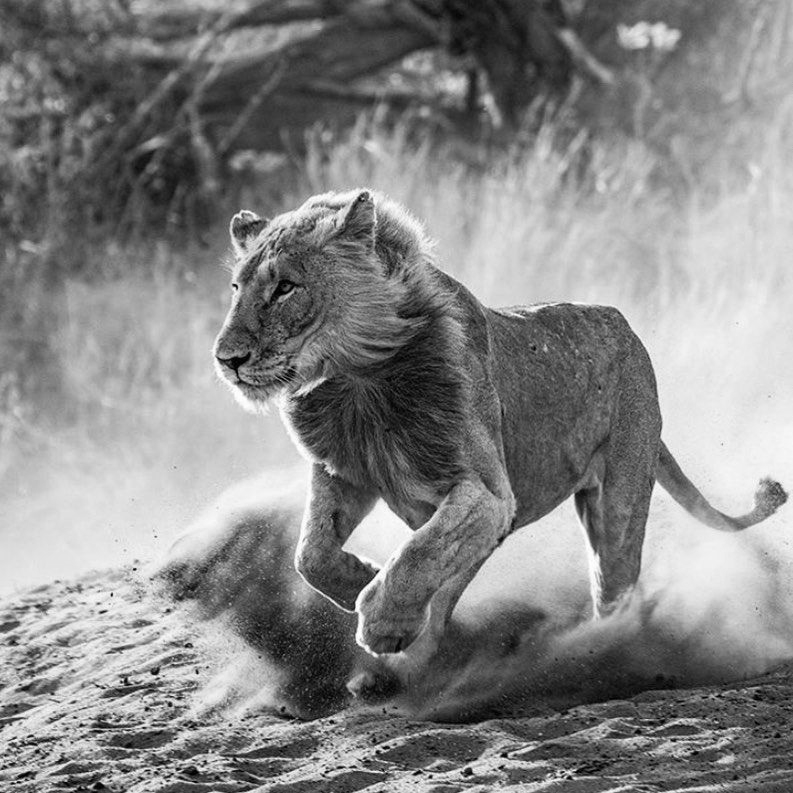
\includegraphics[width=.7\linewidth]{../images/leaopb.png}
      \caption{Imagem original (793x793) }
      \label{fig:sub1}
    \end{subfigure}%
    \begin{subfigure}{.33\textwidth}
      \centering
      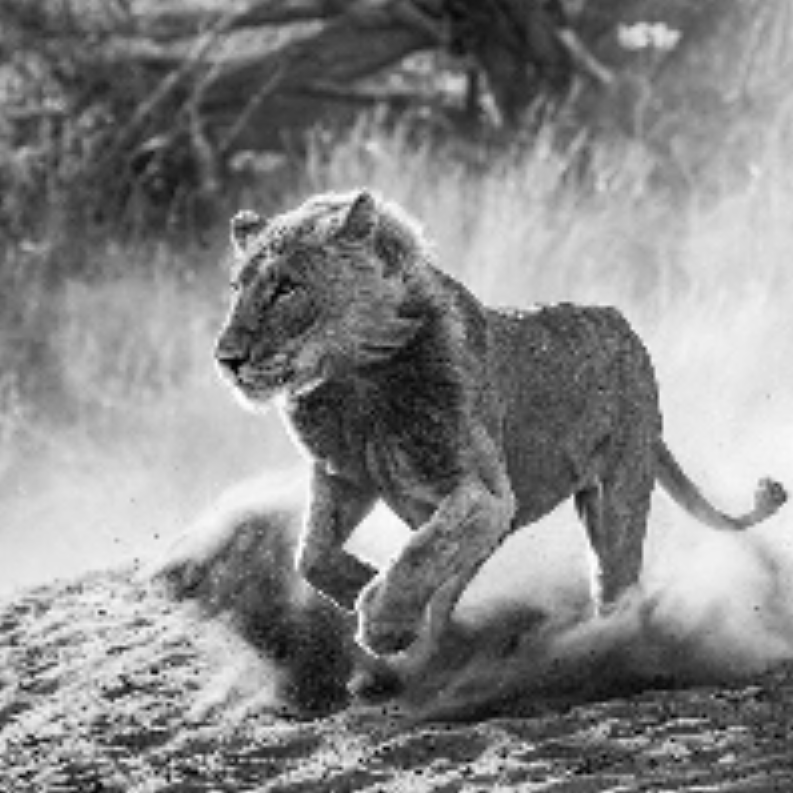
\includegraphics[width=.7\linewidth]{../images/leaopb_bil.png}
      \caption{Método bilinear com $k = 3$}
      \label{fig:sub2}
    \end{subfigure}
    \begin{subfigure}{.33\textwidth}
        \centering
        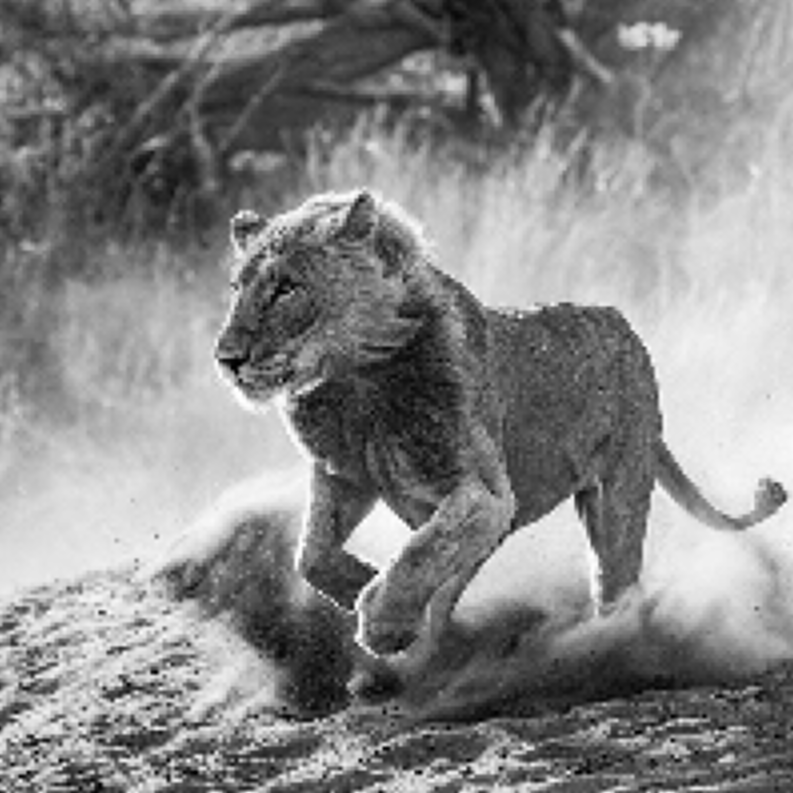
\includegraphics[width=.7\linewidth]{../images/leaopb_bic.png}
        \caption{Método bicúbico com $k = 3$}
        \label{fig:sub1}
      \end{subfigure}%
    \caption{Erro: 0.020500 e 0.020921}
    \label{fig:test}
\end{figure}

\begin{figure}[H]
    \centering
    \begin{subfigure}{.33\textwidth}
      \centering
      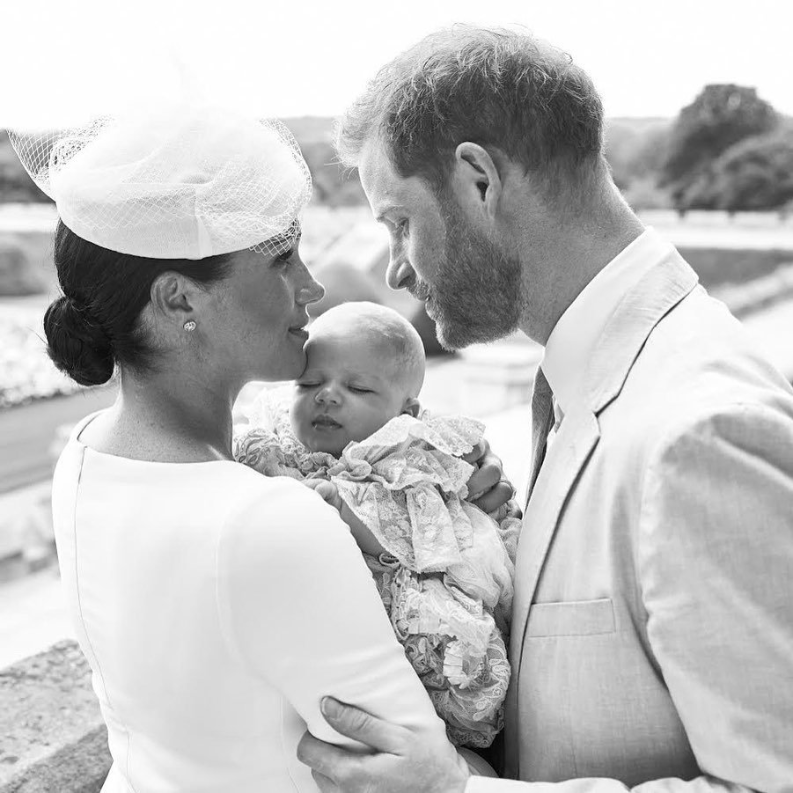
\includegraphics[width=.7\linewidth]{../images/principe.png}
      \caption{Imagem original (793x793) }
      \label{fig:sub1}
    \end{subfigure}%
    \begin{subfigure}{.33\textwidth}
      \centering
      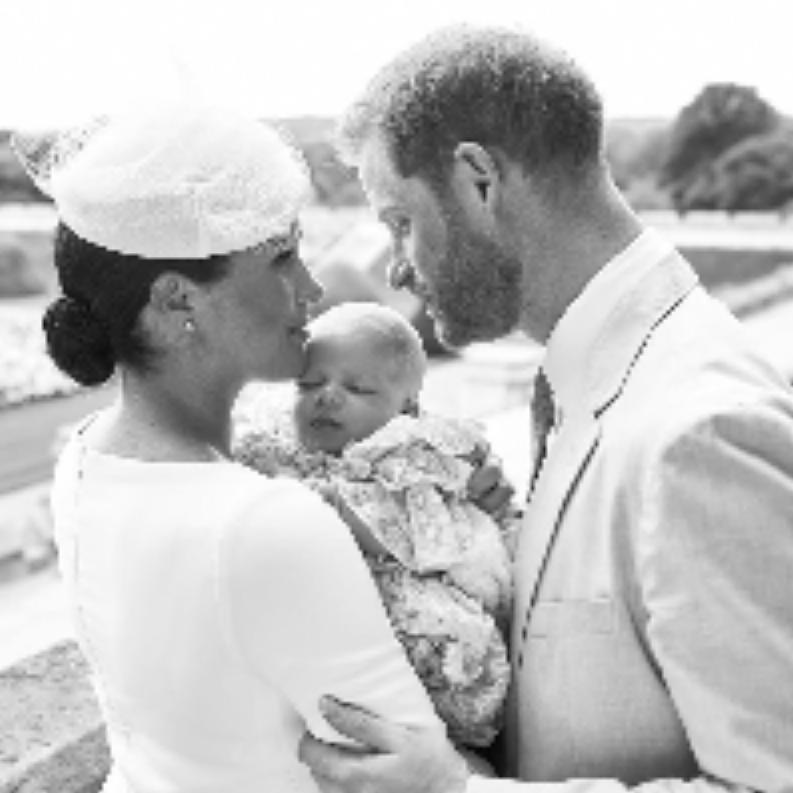
\includegraphics[width=.7\linewidth]{../images/principe_bil.png}
      \caption{Método bilinear com $k = 3$}
      \label{fig:sub2}
    \end{subfigure}
    \begin{subfigure}{.33\textwidth}
        \centering
        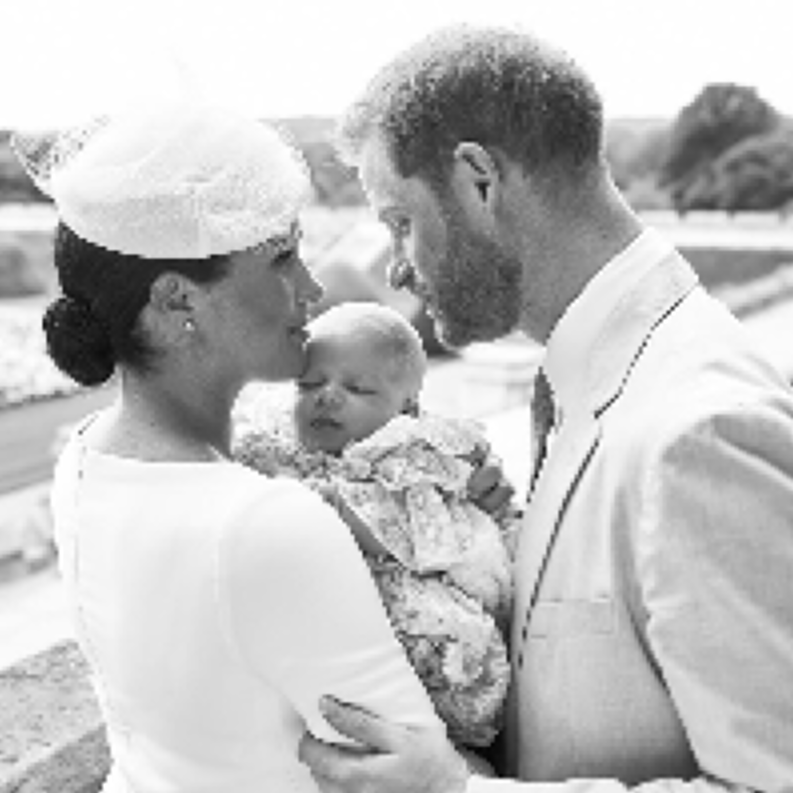
\includegraphics[width=.7\linewidth]{../images/principe_bic.png}
        \caption{Método bicúbico com $k = 3$}
        \label{fig:sub1}
      \end{subfigure}%
    \caption{Erro: 0.0067670 e 0.0067729}
    \label{fig:test}
\end{figure}

\subsubsection*{Imagens coloridas}

\begin{figure}[H]
    \centering
    \begin{subfigure}{.33\textwidth}
      \centering
      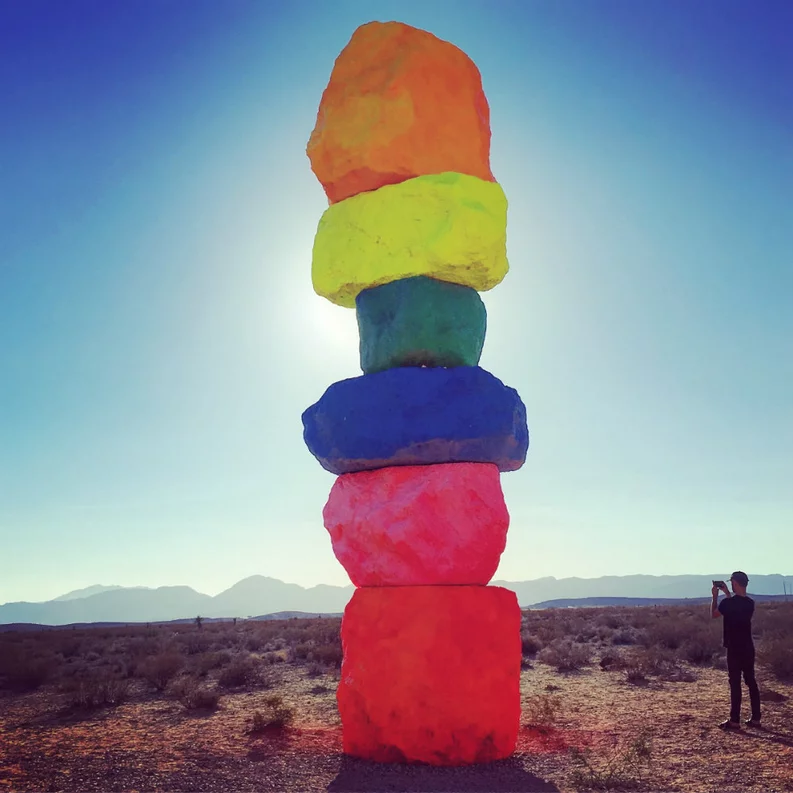
\includegraphics[width=.7\linewidth]{../images/pedrascoloridas.png}
      \caption{Imagem original (793x793) }
      \label{fig:sub1}
    \end{subfigure}%
    \begin{subfigure}{.33\textwidth}
      \centering
      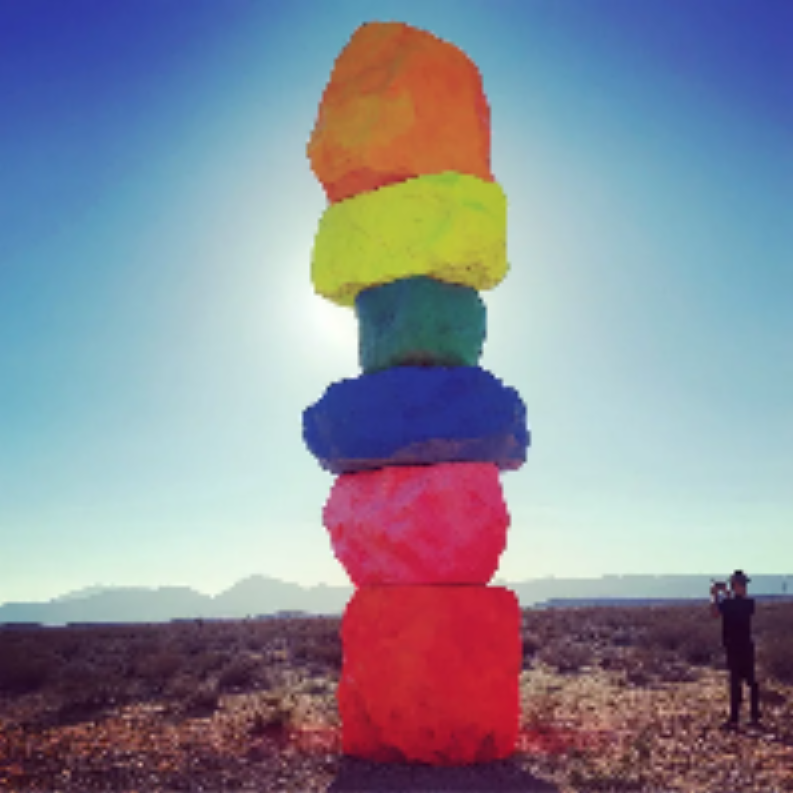
\includegraphics[width=.7\linewidth]{../images/pedrascoloridas_bil.png}
      \caption{Método bilinear com $k = 3$}
      \label{fig:sub2}
    \end{subfigure}
    \begin{subfigure}{.33\textwidth}
        \centering
        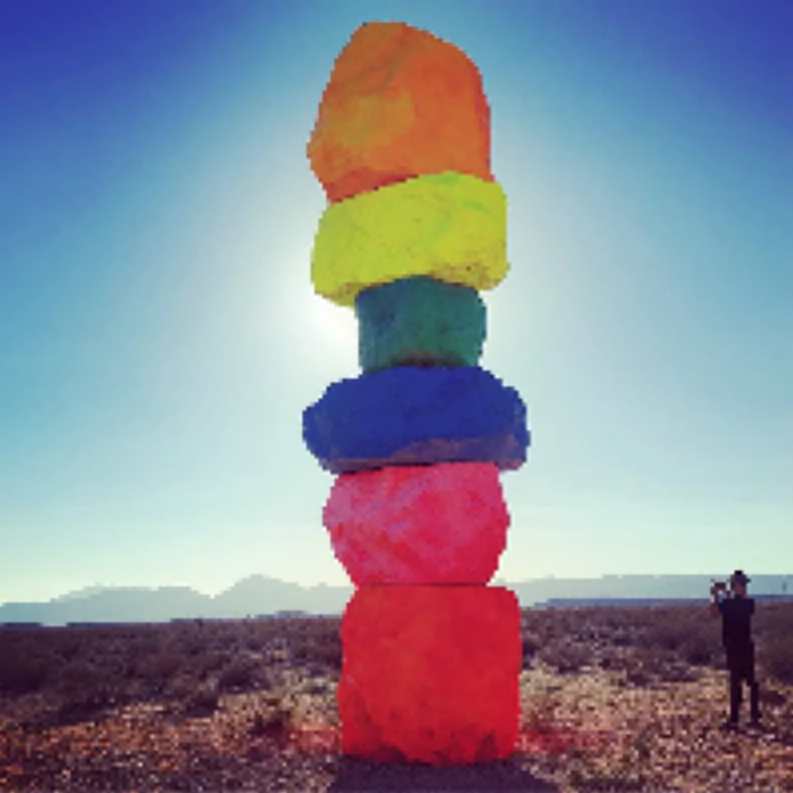
\includegraphics[width=.7\linewidth]{../images/pedrascoloridas_bic.png}
        \caption{Método bicúbico com $k = 3$}
        \label{fig:sub1}
      \end{subfigure}%
    \caption{Erro: 0.010588 e 0.011070}
    \label{fig:test}
\end{figure}

\begin{figure}[H]
    \centering
    \begin{subfigure}{.33\textwidth}
      \centering
      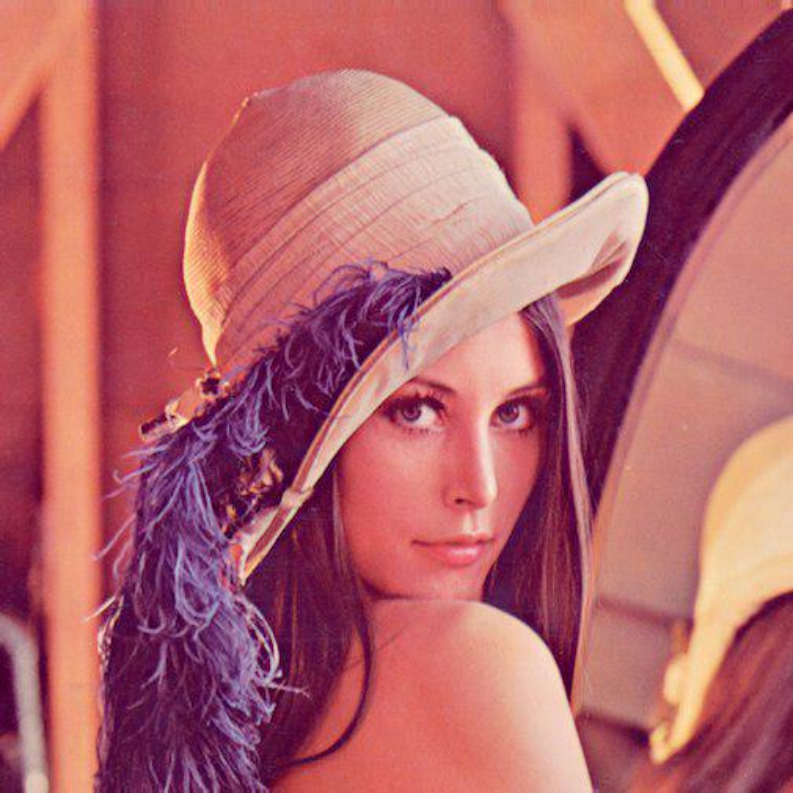
\includegraphics[width=.7\linewidth]{../images/lena.png}
      \caption{Imagem original (793x793) }
      \label{fig:sub1}
    \end{subfigure}%
    \begin{subfigure}{.33\textwidth}
      \centering
      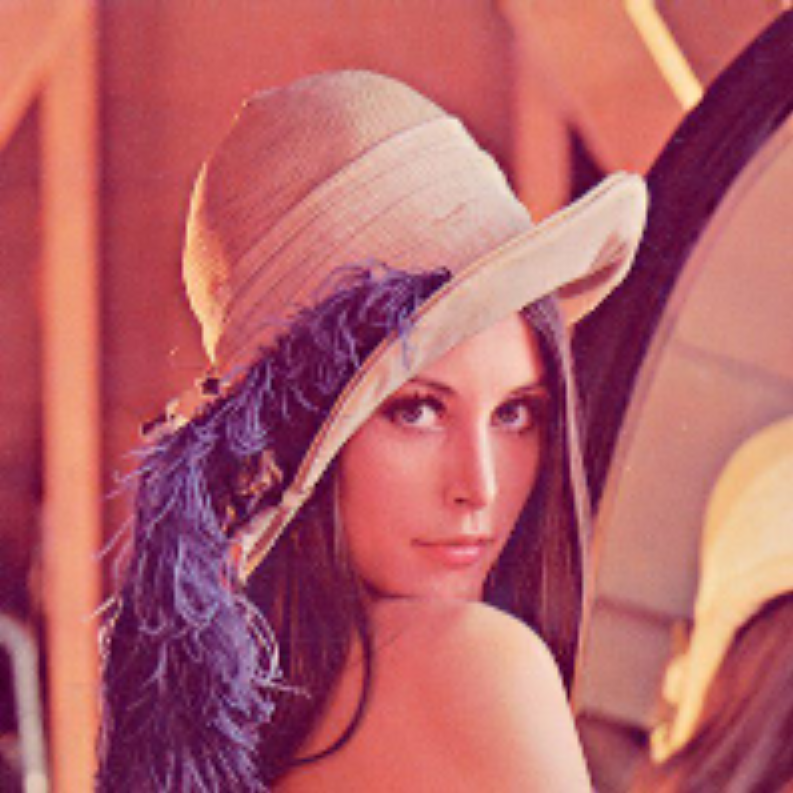
\includegraphics[width=.7\linewidth]{../images/lena_bil.png}
      \caption{Método bilinear com $k = 3$}
      \label{fig:sub2}
    \end{subfigure}
    \begin{subfigure}{.33\textwidth}
        \centering
        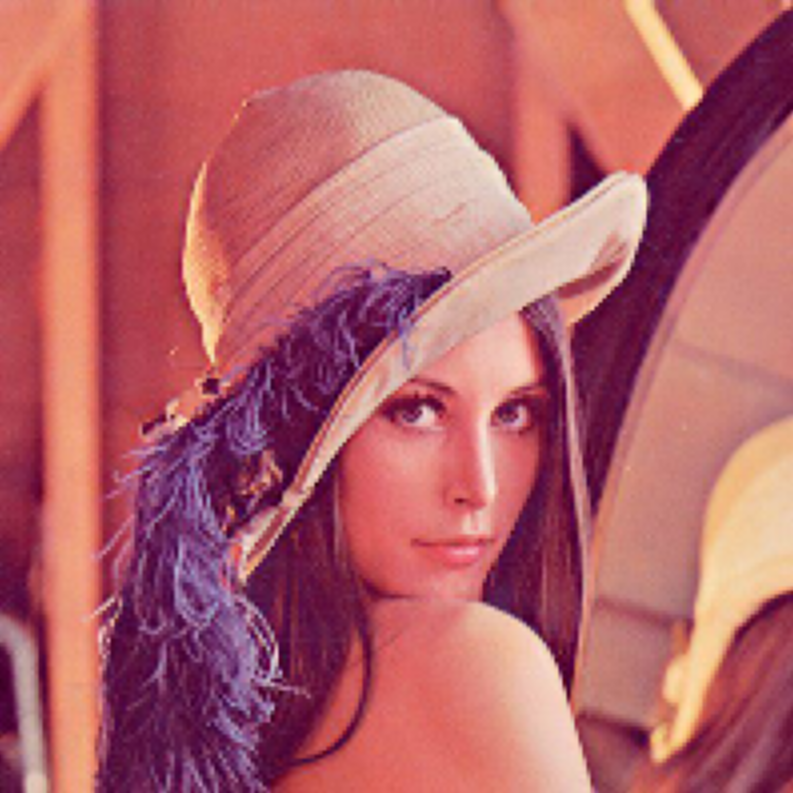
\includegraphics[width=.7\linewidth]{../images/lena_bic.png}
        \caption{Método bicúbico com $k = 3$}
        \label{fig:sub1}
      \end{subfigure}%
    \caption{Erro: 0.00983 e 0.0095212}
    \label{fig:test}
\end{figure}

\begin{itemize}
    \item \textbf{Funciona bem para imagens preto e branco?} \\
        Funcionou muito bem para imagens preto e branco, muito melhor do que
        para imagens geradas por funções na seção anterior.

    \item \textbf{Funciona bem para imagens coloridas?} \\
        Novamente, funcionou muito bem para imagens coloridas, muito melhor do que
        para imagens geradas por funções na seção anterior.

    \item \textbf{Como o valor de h muda a interpolação?} \\
        Testei com diversos valores de $h$ e o erro não mudou significativamente.
    
    \item \textbf{Como se comporta o erro?} \\
        O erro aumentou um pouco em alguns casos conforme $k$ aumentou, se manteve praticamente
        estável conforme $h$ variou, e de forma geral foi um pouco maior para imagens
        coloridas. Acredito que o erro grande nessas imagens geradas por funções
        pode ser devido a mudanças bruscas na cor, como podemos observar nas imagens,
        não há uma suavidade nas transições como existe em imagens reais.

        Outra coisa que notei é que as vezes uma diferença pequena no erro é
        visualmente bem grande, como no exemplo abaixo. 
        
        \begin{figure}[H]
          \centering
          \begin{subfigure}{.45\textwidth}
            \centering
            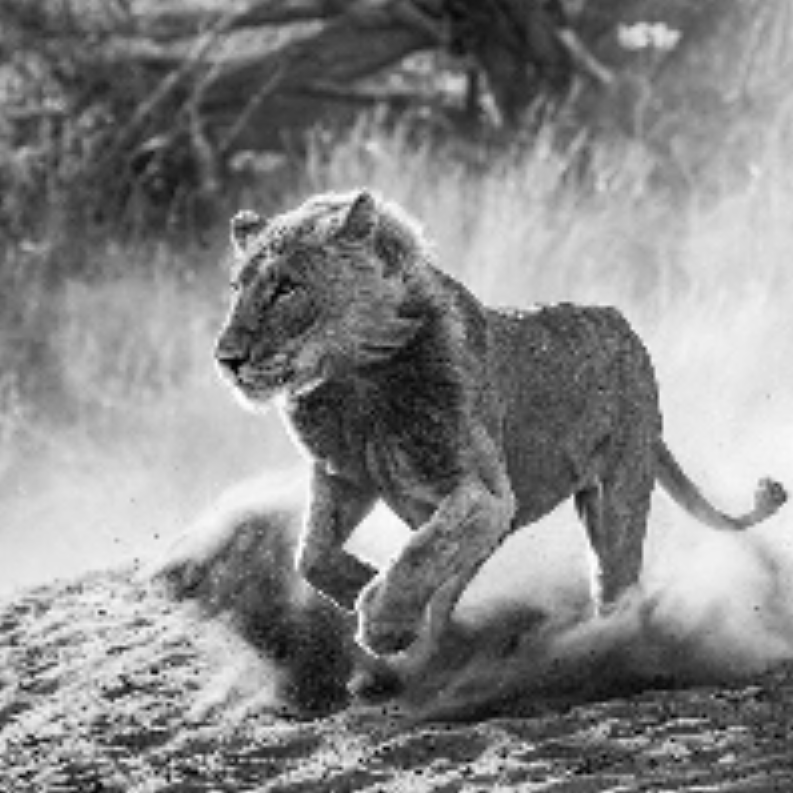
\includegraphics[width=.7\linewidth]{../images/leaopb_k3.png}
            \caption{Método bilinear com $k = 3$}
            \label{fig:sub2}
          \end{subfigure}
          \begin{subfigure}{.45\textwidth}
              \centering
              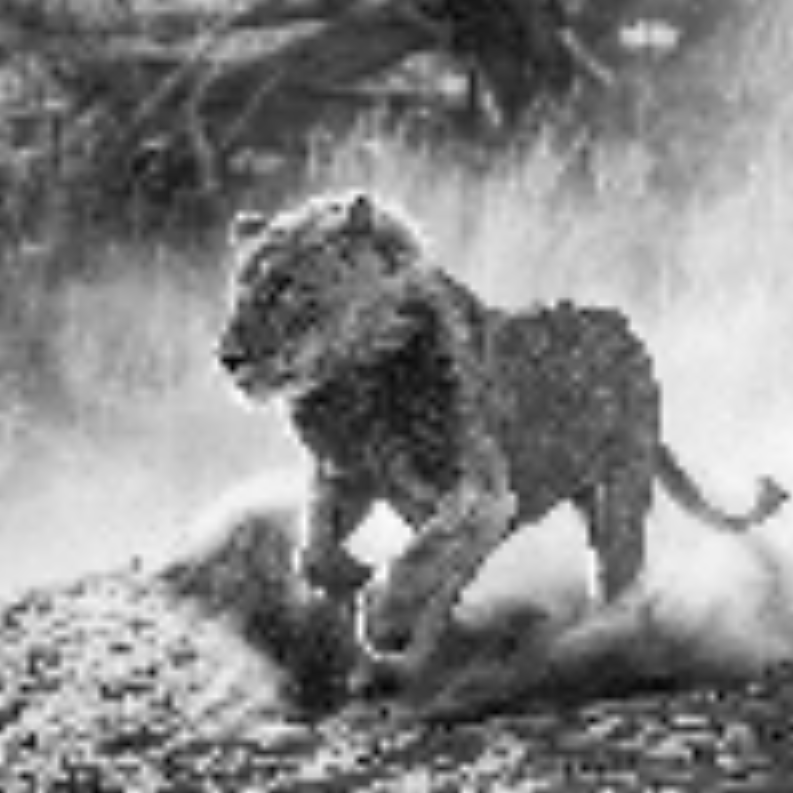
\includegraphics[width=.7\linewidth]{../images/leaopb_k7.png}
              \caption{Método bilinear com $k = 7$}
              \label{fig:sub1}
            \end{subfigure}%
          \caption{Erro: 0.020500 e 0.030992}
          \label{fig:test}
      \end{figure}

    \item \textbf{Comparação $k = 7$ e $k = 1$ três vezes} \\
        O erro ficou muito parecido em ambos os casos nos meus testes, até mesmo
        iguais em alguns testes. Segue um exemplo:

      \begin{figure}[H]
          \centering
          \begin{subfigure}{.45\textwidth}
            \centering
            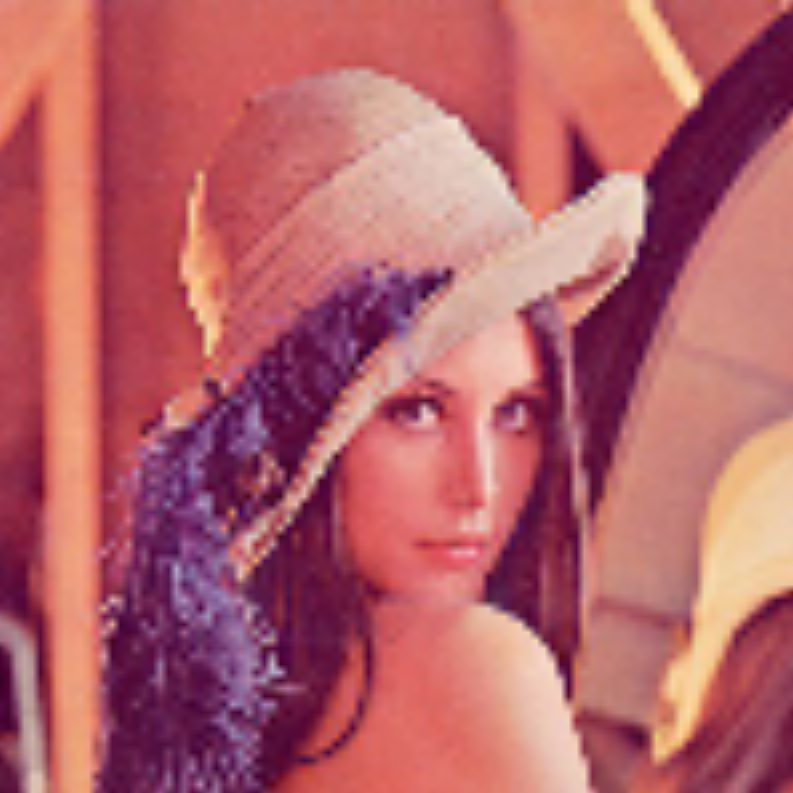
\includegraphics[width=.7\linewidth]{../images/lena_k7x1.png}
            \caption{Método bilinear com $k = 7$}
            \label{fig:sub2}
          \end{subfigure}
          \begin{subfigure}{.45\textwidth}
              \centering
              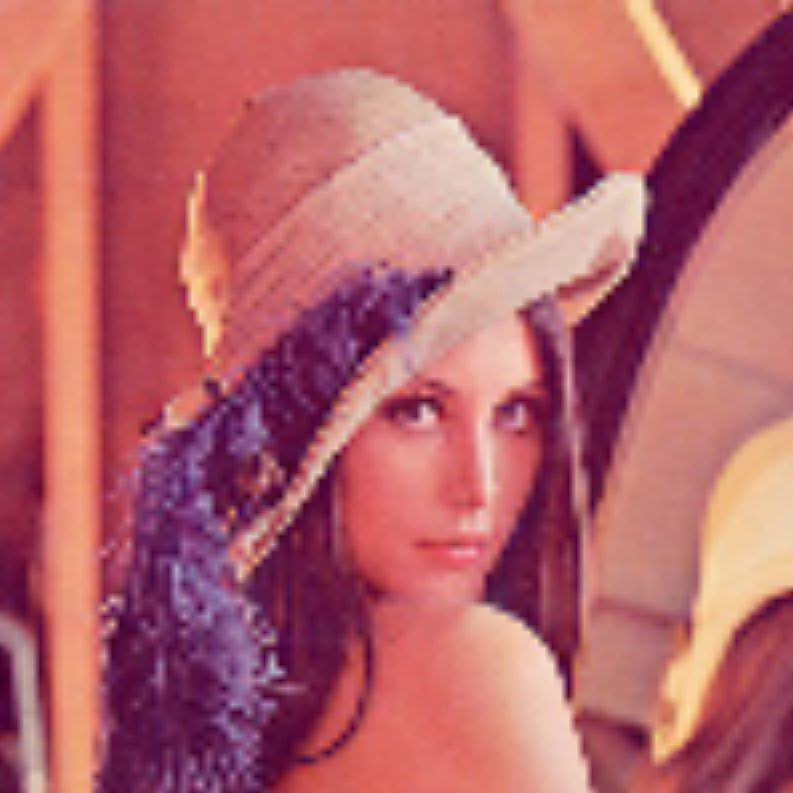
\includegraphics[width=.7\linewidth]{../images/lena_k1x3.png}
              \caption{Método bilinear com $k = 1$ três vezes}
              \label{fig:sub1}
            \end{subfigure}%
          \caption{Erro: 0.022366 e 0.022344}
          \label{fig:test}
      \end{figure}
\end{itemize}

\end{document}